\section{The two cost laws: a line and a staircase}
\label{sec:laws}

\subsection{Parallel formulation}

The intuition is simple: AR pays per token, DG pays per block. Every
output token on an AR model triggers a fresh forward pass over a
growing KV cache --- the cost is strictly linear. A block-diffusion
model denoises an entire canvas of $C$ tokens in parallel through $K$
steps, then steps to the next canvas --- the cost is flat inside a
block and jumps only at the boundary. Both architectures decode
output tokens from the same prompt, but their costs accumulate
differently.

In general form, both cost laws share the structure:
\begin{equation}
\label{eq:general}
T = a + b \cdot f(L_{\mathrm{out}})
\end{equation}
where:
\begin{itemize}[nosep]
\item $T$ is the per-event latency in milliseconds,
\item $L_{\mathrm{out}}$ is the output length in tokens,
\item $a$ is the fixed cost (intercept / floor) independent of output
  length,
\item $b$ is the marginal cost per unit of output,
\item $f(L_{\mathrm{out}})$ is the output-length function: linear for
  AR ($f = L_{\mathrm{out}}$), staircase for DG
  ($f = \lceil L_{\mathrm{out}}/C \rceil - 1$),
\item $C$ is the canvas size (tokens per block, $C = \canvasLength$ for
  DiffusionGemma),
\item $K$ is the number of denoising steps per canvas ($K = 8$ at the
  operating point).
\end{itemize}

The measured cost laws are:
\begin{align}
\label{eq:ar}
T_{\textsc{ar}}(L_{\mathrm{out}}) &= \arBase + \arSlope \cdot L_{\mathrm{out}} && \text{(ms, linear)} \\
\label{eq:dg}
T_{\textsc{dg}}(L_{\mathrm{out}}) &= \dgBase + \dgStep \cdot \Bigl(\bigl\lceil \tfrac{L_{\mathrm{out}}}{\canvasLength}\bigr\rceil - 1\Bigr) && \text{(ms, staircase)}
\end{align}

For AR: $a = \arBase$\,ms is the prompt prefill cost (amortised by prefix
caching). The low value reflects the MoE architecture's efficient
prefill: only 3\,B of 30\,B parameters are active per token, so the
prefill computation is much cheaper than for a dense model of comparable
total size. $b = \arSlope$\,ms is the per-token decode cost --- one KV
cache forward pass per token. Every output token costs exactly $b$,
regardless of position.

For DG: $a = \dgBase$\,ms (first-canvas cost: prompt prefill paid $K$
times, once per denoising step, plus $K$ denoising passes over $C$
tokens). $b = \dgStep$\,ms (marginal cost of one additional canvas ---
a fresh denoising pass over a new block of $C$ tokens). Within a
canvas, $b = 0$: additional tokens are free because they are denoised
in parallel. This is why $a$ is much larger for DG than AR, while $b$
is zero within a block.

The operating point $K{=}8$ was selected as the latency/quality knee:
quality is approximately flat above $K{=}8$ (0.853 at $K{=}8$, 0.862 at $K{=}32$; the $+0.009$ rise is at the edge of the $n{=}200$ standard error)
while latency saturates above $K{=}16$. Each additional canvas costs
\dgStep\,ms (median of 7 measured transitions, range
\dgStepLo--\dgStepHi).

The key structural difference: within a canvas, DG emits tokens for free
(parallel denoising), while AR pays $\arSlope$\,ms per token. At canvas
boundaries, DG pays a fixed $\dgStep$\,ms step, while AR's cost is
unaffected. AR is a metered taxi: the fare climbs with every block.
DG is a subway: flat fare per station, no matter how many tokens board.
The shapes cross where the two costs are equal
($T_{\textsc{ar}} = T_{\textsc{dg}}$). Solving for $L_{\mathrm{out}}$:
\begin{equation}
\label{eq:lcross}
L^{*} = \frac{a_{\textsc{dg}} - a_{\textsc{ar}}}{b_{\textsc{ar}}}
= \frac{\dgBase - \arBase}{\arSlope} = \crossoverL \text{ tokens},
\qquad
\lambda^{*} = \frac{1000}{a_{\textsc{dg}}} = \frac{1000}{\dgBase} = \crossoverLambda \text{ events/s}
\end{equation}
where $L^{*}$ is the output length at which both architectures produce
equal latency (the crossover point), $a_{\textsc{ar}}$ and
$a_{\textsc{dg}}$ are the fixed costs (intercepts) from
Eqs.~\ref{eq:ar}--\ref{eq:dg}, $b_{\textsc{ar}}$ is the AR per-token
slope, and $\lambda^{*}$ is the maximum serial event rate before a
queue forms (the reciprocal of the DG floor $a_{\textsc{dg}}$, in
events per second). Below $L^{*}$, AR is cheaper; above it, DG is ---
until the next canvas edge, where the gap widens again.

\begin{figure}[t]
\centering
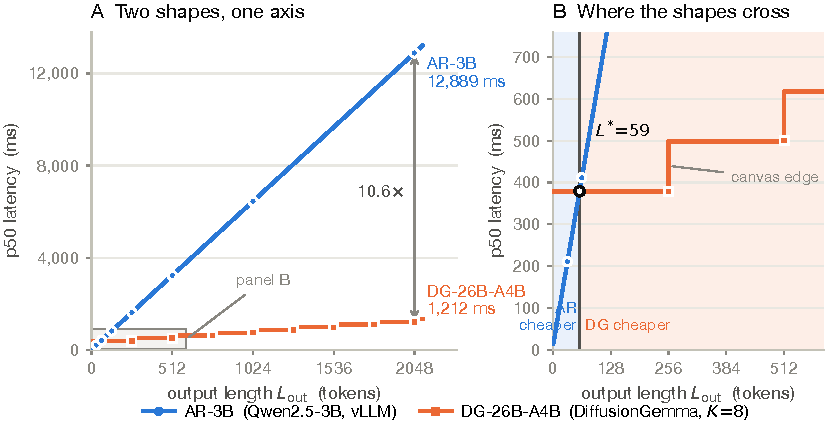
\includegraphics[width=\linewidth]{figures/fig1_cost_shapes.pdf}
\caption{The two cost shapes. AR latency grows linearly with output
length (each token costs $\arSlope$\,ms); DG latency is a staircase
that steps by $\dgStep$\,ms at every 256-token canvas boundary and is
flat inside. The gap widens with $L$ because AR's line has no floor
while DG's staircase is bounded. AR values from the fitted cost law
(Eq.~\ref{eq:ar}), extrapolated beyond natural EOS at $\sim$123
tokens; DG measured (BGL, $n{=}200$, $K{=}8$). The measured ratio
at $L{=}256$ is $15.6\times$ (Table~\ref{tab:niche}).}
\label{fig:shapes}
\end{figure}

\begin{figure}[t]
\centering
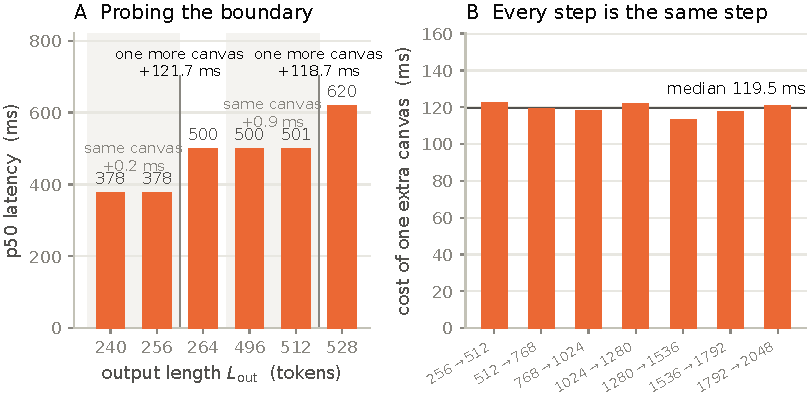
\includegraphics[width=\linewidth]{figures/fig2_canvas_edges.pdf}
\caption{The staircase probed at canvas boundaries ($K{=}8$, BGL,
$n{=}200$). \textbf{A:} latency is flat inside a canvas and jumps
$\sim$120\,ms at the boundary --- tokens within a canvas are free.
\textbf{B:} all seven canvas transitions out to $L{=}2048$ cost the
same within noise (range \dgStepLo--\dgStepHi\,ms, median \dgStep\,ms),
confirming the staircase is regular: every canvas costs the same
regardless of position.}
\label{fig:edges}
\end{figure}

\subsection{What the base is made of}

The \dgBase\,ms base is 37--53\% prefill (by linear interpolation
between $K{=}2$ and $K{=}8$; see Appendix~\ref{app:decomp}). Each
denoising step re-attends the full prompt, so prefill is paid $K$ times.
If the prompt KV were cached across denoising steps, the base could fall
toward $\sim$150\,ms and $L^{*}$ would move downward. We treat the
measured base as the operative number; see Appendix~\ref{app:forced} for
the asymmetry with the batching caveat.

\subsection{Generalisation}

Both laws generalise from BGL to HDFS within 1.7\%. The AR
generalisation was measured on the dense AR-3B (not AR-30B); the DG
canvas step moves from \bglStep\,ms to \hdfsStep\,ms ($+1.7\%$).
